\documentclass[a4paper]{scrreprt}
\usepackage{xcolor}                % we use grey text here
\usepackage{graphicx}              % figures
\usepackage{listings}              % source code
\usepackage{hyperref}              % navigation
\usepackage{bold-extra}            % bold keywords in listings
\usepackage[small]{caption}        % better-looking captions
\parindent0mm                      % this looks better in short paragraphs

% some colors
\definecolor{arggrey}{gray}{.6}
\definecolor{middlegray}{gray}{.5}

% listings style
\lstset{
  basicstyle=\scriptsize\ttfamily,
  keywordstyle=\bfseries\ttfamily,
  commentstyle=\color{middlegray}\ttfamily,
  showstringspaces=false,
  flexiblecolumns=false,
  tabsize=2,
  numbers=left,
  numberstyle=\tiny,
  numberblanklines=false,
  stepnumber=1,
  numbersep=10pt,
  xleftmargin=15pt
}

% this is a basic language definition for the listings package
\lstdefinelanguage{Lua}
{
 morecomment = [l]{--},
 morecomment = [s]{--[*[}{]*]--},
 morestring=[b]",
 morestring=[b]',
 sensitive = true,
 morekeywords = {and, break, do, else, elseif, end, for,
    function, if, local, nil, not, or, repeat, return, then,
    until, while}
 morekeywords=[2]{},
}

\title{The \emph{AnnotationSketch} genome annotation drawing library}
\subject{Supplementary Information}
\author{Sascha Steinbiss, Gordon Gremme, Christin Sch\"arfer, Malte Mader\\ and Stefan Kurtz}

\begin{document}

\maketitle

\tableofcontents

\chapter{AnnotationSketch}

The \emph{AnnotationSketch} module is a versatile and efficient C-based drawing library for GFF3-compatible genomic annotations. It is included in the \emph{GenomeTools} distribution.

\section{Overview}
\emph{AnnotationSketch} consists of several classes, which take part in
three visualization \emph{phases} (see Fig. \ref{dataflow}).

\begin{figure}[ht]
\centering{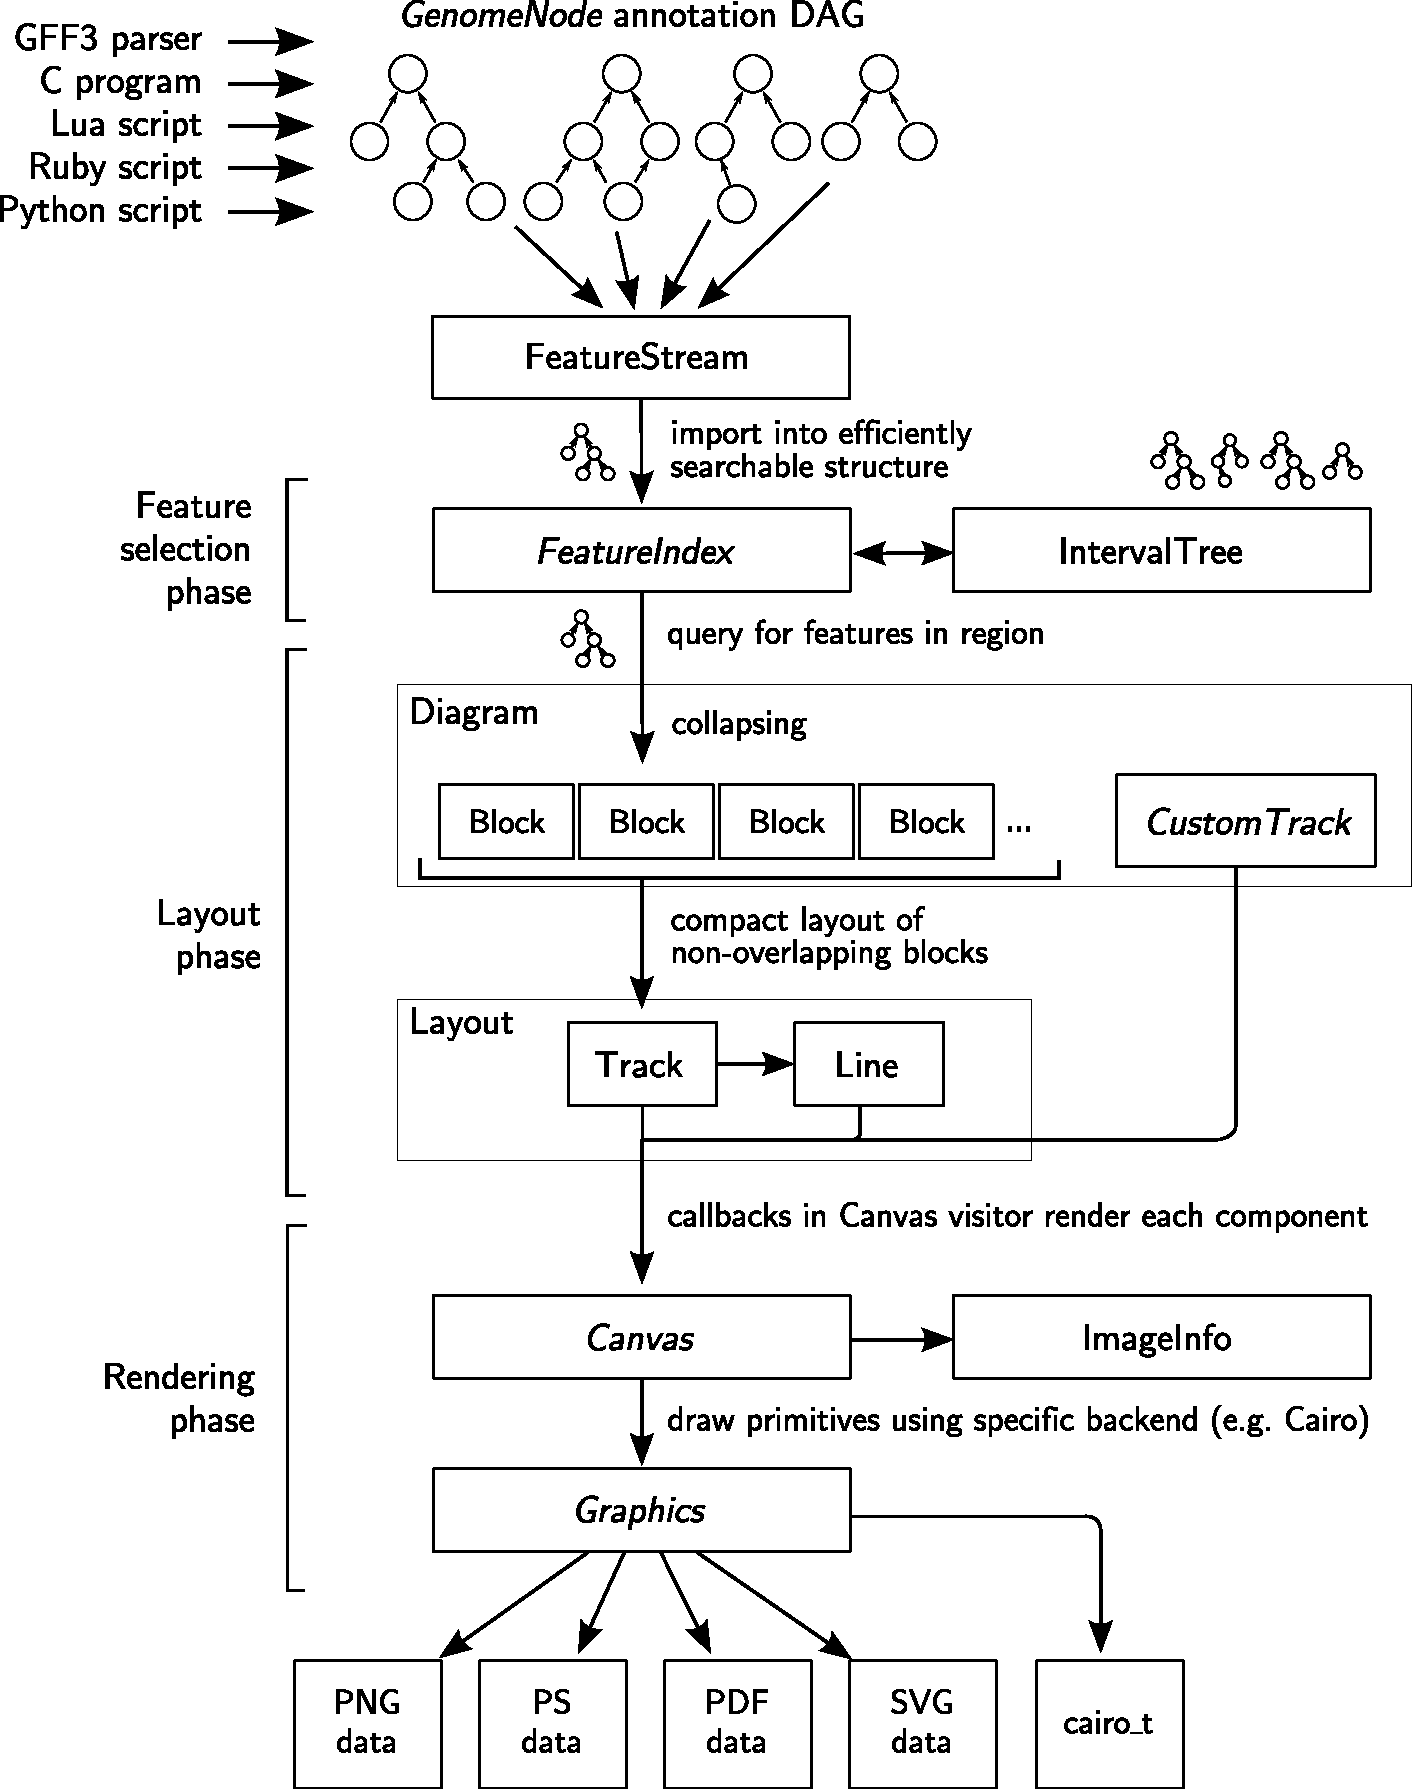
\includegraphics[width=.9\textwidth]{../../www/genometools.org/htdocs/images/dataflow.pdf}}
\caption{Schematic of the data flow through the classes involved in image creation.}
\label{dataflow}
\end{figure}

\subsection{Phase 1: Feature selection}
The GFF3 input data are parsed into a directed acyclic graph (\emph{annotation graph}, see Fig. \ref{gfftree} for an example) whose nodes are single features (lines from the GFF3 file). Edges represent the \emph{part-of} relationships between
groups of genomic features according to the
Sequence Ontology hierarchy. A validating GFF3 parser is available in \emph{GenomeTools}. GFF3 files \emph{must} be valid according to the GFF3 specification to ensure that they can be read for \emph{AnnotationSketch} drawing.

\begin{figure}[ht]
\centering{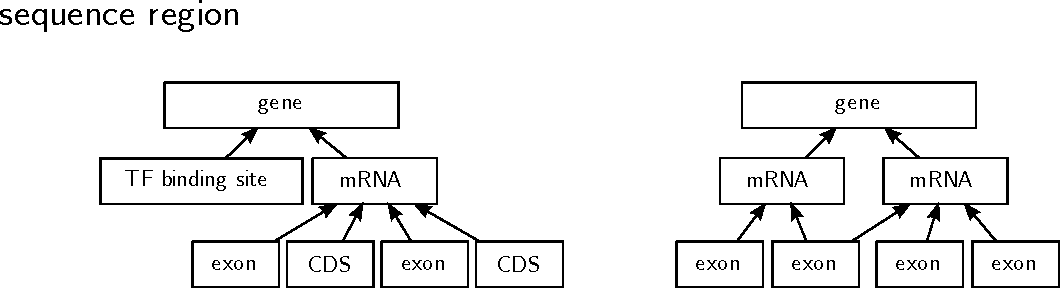
\includegraphics[width=.9\textwidth]{../../www/genometools.org/htdocs/images/gfftree.pdf}}
\caption{Example sequence region containing two genes in an annotation graph depicting the \emph{part-of} relationships between their components.}
\label{gfftree}
\end{figure}
Each top-level node is then registered into a persistent \emph{FeatureIndex} object that can be (repeatedly) queried for all the features in a genomic region of interest. Alternatively, annotation graphs can be built by the user by creating each node explicitly and then connecting the nodes in a way such that the relationships are reflected in the graph structure (see examples section for example annotation graph building code).

\subsection{Phase 2: Layout}
The next step consists of processing the features (given via a \emph{FeatureIndex} or a simple array of top level nodes) into a structural \emph{Diagram} object which first builds \emph{blocks} from features by grouping and overlaying them according to several options (see Collapsing). During image generation, the \emph{Block} objects are distributed into \emph{Line} (each containing non-overlapping blocks) and \emph{Track} objects (containing all lines of a given type). \emph{Tracks} and \emph{Lines} are contained within the \emph{Diagram} object and correspond to particular building blocks of the resulting diagram (see Fig. \ref{diagram}). The overall layout of the diagram tries to keep the amount of vertical space as compact as possible. How new \emph{Lines} are created depends on the chosen  implementation of the \emph{LineBreaker} interface, by default a \emph{Block} is pushed into a new \emph{Line} when either the \emph{Block} or its caption overlaps with another one.

\begin{figure}[ht]
\centering{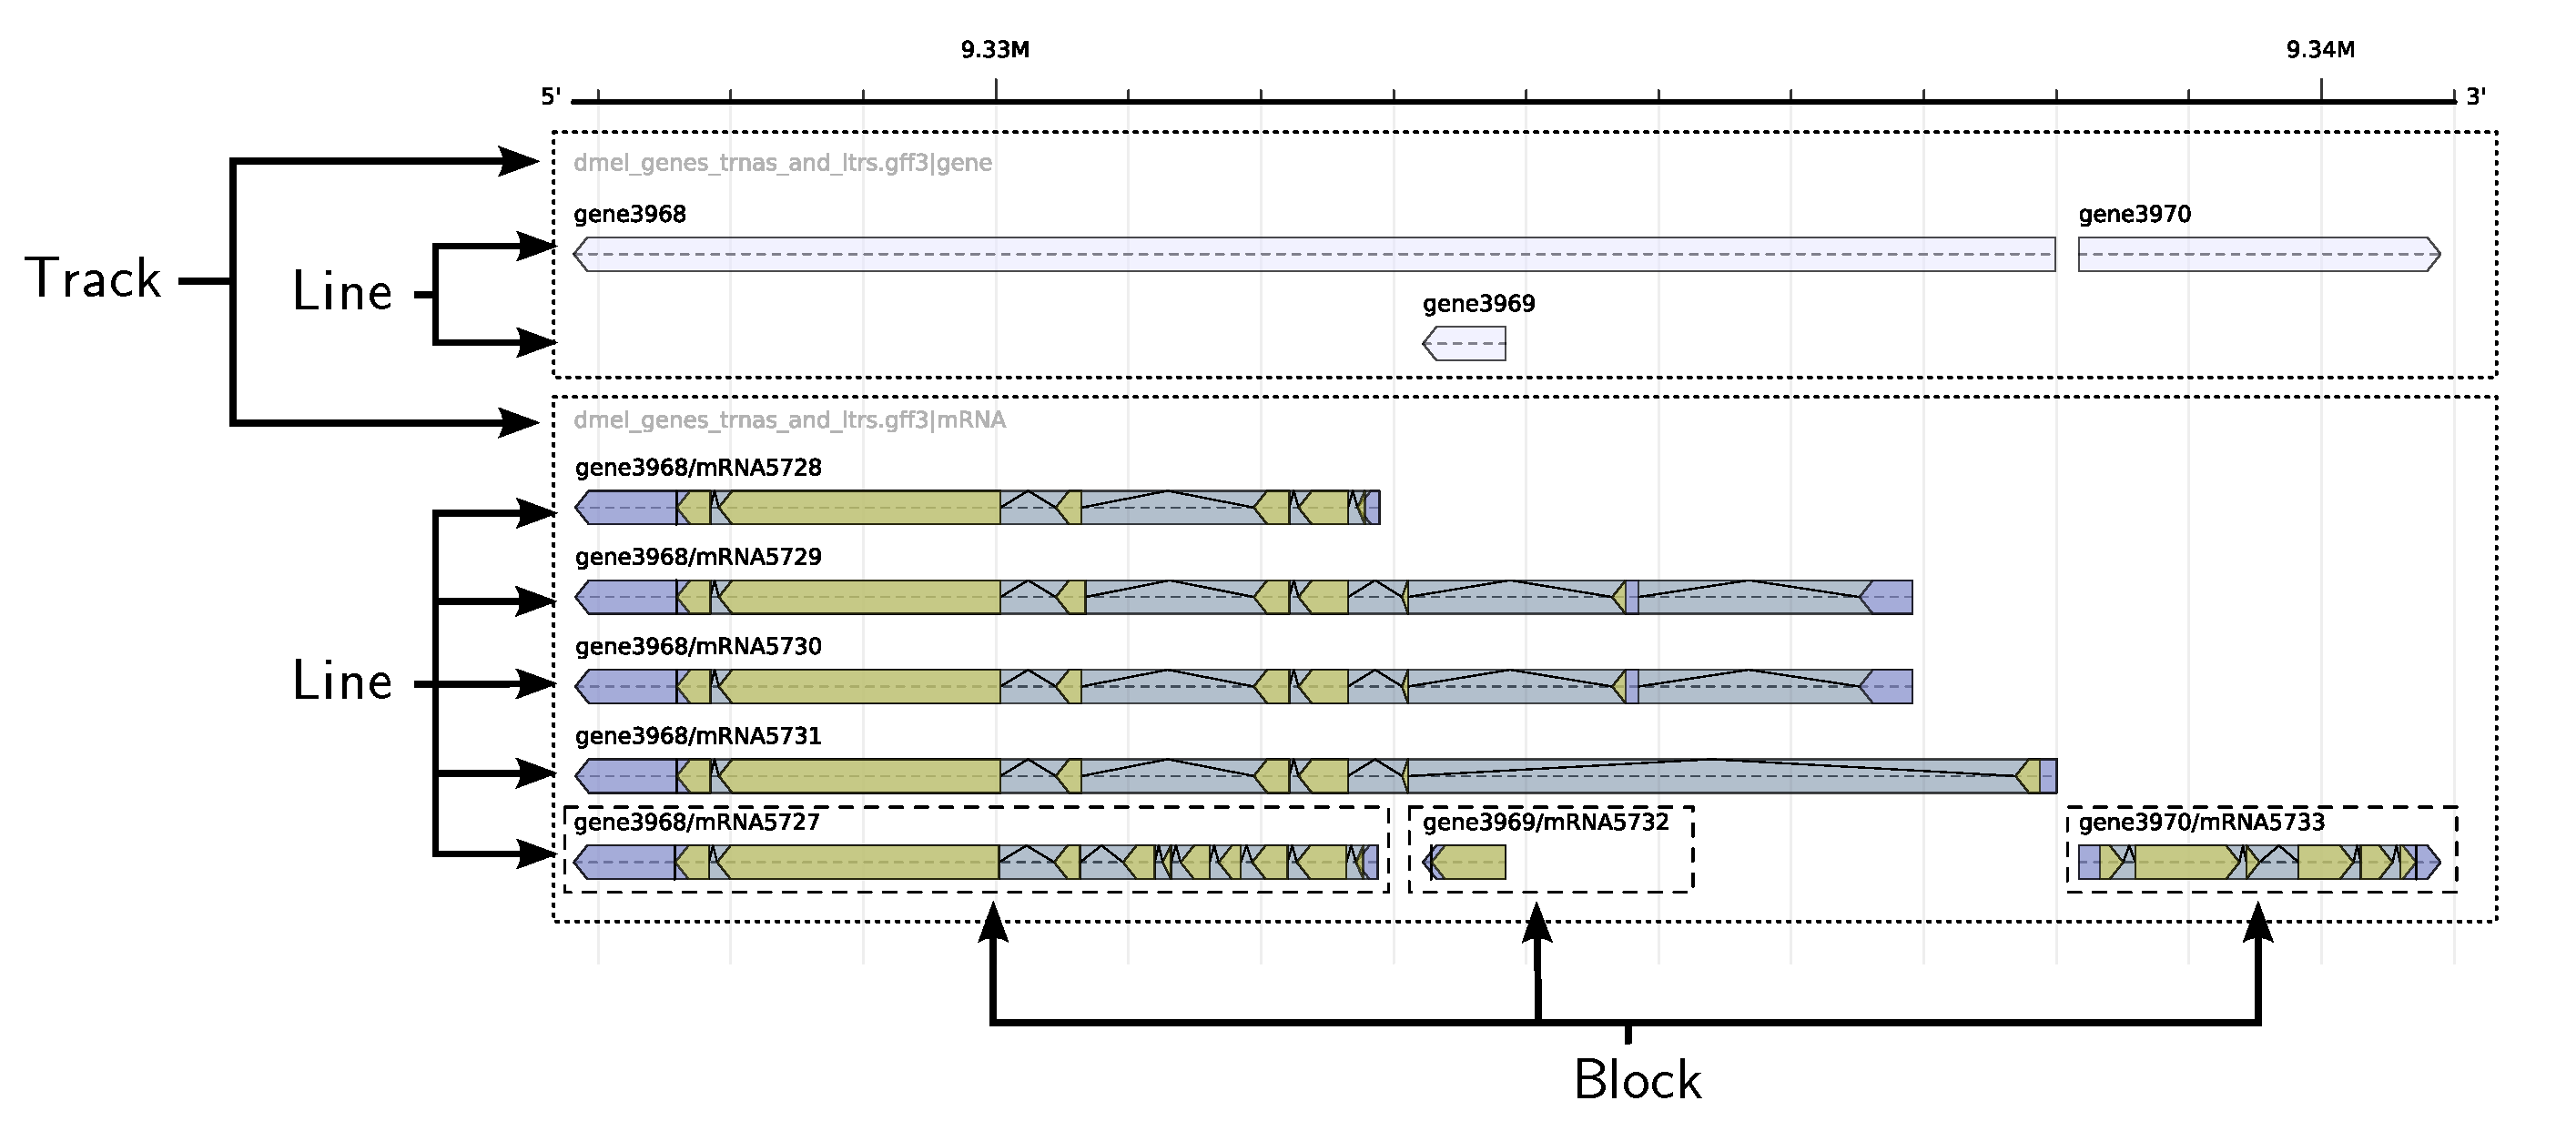
\includegraphics[width=\textwidth]{../../www/genometools.org/htdocs/images/diagram.pdf}}
\caption{The components of the \emph{Diagram} class reflect sections of the resulting image.}
\label{diagram}
\end{figure}

\subsection{Phase 3: Rendering}
In the final phase, the \emph{Diagram} object is used as a blueprint to create an
image of a given type and size, considering user-defined options.

Rendering logic is implemented in the \emph{Canvas} class, whose methods are called during traversal of the \emph{Diagram} structure. It encapsulates the state of a drawing and works independently of the chosen rendering back-end. Instead, rendering back-end-dependent subclasses of \emph{Canvas} are closely tied to a specific implementation of the \emph{Graphics} interface, whose implementations provides methods to draw a number of primitives to a drawing surface abstraction. The \emph{Graphics} interface implementations wrap around a low-level graphics library, allowing for easy extension or replacement of the graphics back-end. Currently, there is a \emph{Graphics} implementation for the Cairo 2D graphics library (\emph{GraphicsCairo}) and two \emph{Canvas} subclasses providing access to the image file formats supported by Cairo (\emph{CanvasCairoFile}) and to arbitrary Cairo contexts (\emph{CanvasCairoContext}, which directly accesses a \texttt{cairo\_t}). This class can be used, for example, to directly draw \emph{AnnotationSketch} output in any graphical environment which is supported by Cairo (see  list of supported surface types).



\subsection{Collapsing}
By default, \emph{Lines} are grouped by the Sequence Ontology type associated with the top-level elements of their \emph{Blocks}, resulting in one track per type.
To obtain a shorter yet concise output, tracks for parent types in the feature graph can be enabled to contain all the features of their child types. The features with the given type are then drawn on top of their parent features (e.g. all \emph{exon} and \emph{intron} features are placed into their parent \emph{mRNA} or \emph{gene} track). This process is called \emph{collapsing}. Collapsing can be enabled by setting the \texttt{collapse\_to\_parent} option for the respective child type to \texttt{true}, e.g. the following options:

\begin{lstlisting}[language=Lua, showstringspaces=false,numbers=none,frame=single]
config = {
  exon = {
    ...,
    collapse_to_parent = true,
    ...,
  },
  intron = {
    ...,
    collapse_to_parent = true,
    ...,
  },
  CDS = {
    ...,
    collapse_to_parent = true,
    ...,
  },
}
\end{lstlisting}
would lead to all features of the \emph{exon}, \emph{intron} and \emph{CDS} types collapsing into the \emph{mRNA} track (see Fig. \ref{collapsetypes} and \ref{cnn_large}).

\begin{figure}
\centering{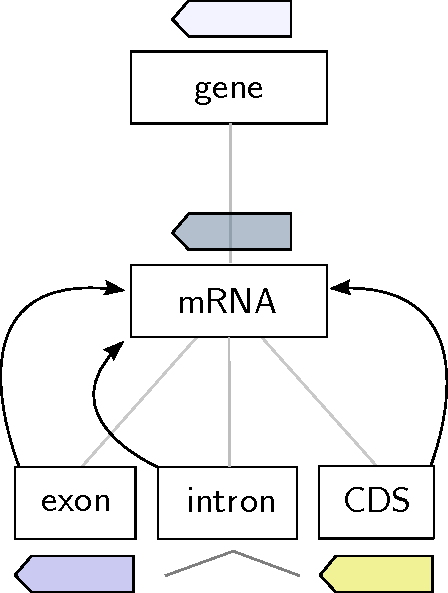
\includegraphics[width=.3\textwidth]{../../www/genometools.org/htdocs/images/collapse_types.pdf}}
\caption{Schematic of the relationships between the \emph{gene}, \emph{mRNA}, \emph{exon}, \emph{intron} and \emph{CDS} types and the colors of their representations in a diagram. The arrows illustrate how the relationships influence the collapsing process if collapsing is enabled for the \emph{exon}, \emph{intron} and \emph{CDS} types. In this example, they will be drawn on top of their parent \emph{mRNA} features.}
\label{collapsetypes}
\end{figure}
\begin{figure}
\centering{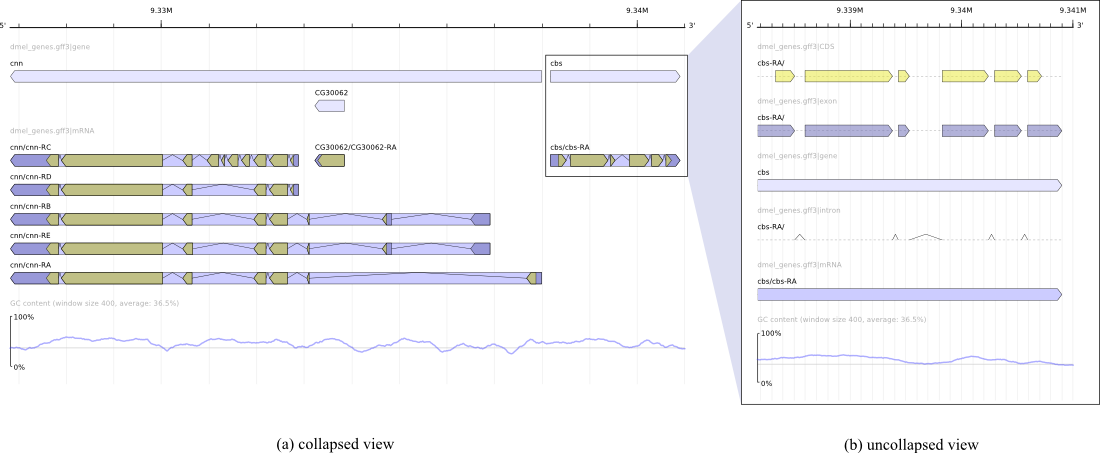
\includegraphics[width=\textwidth]{../../www/genometools.org/htdocs/images/cnn_large}}
\caption{Example image of the \emph{cnn} and \emph{cbs} genes from \emph{Drosophila melanogaster} (Ensembl release 50, positions 9326816--9341000 on chromosome arm 2R) as drawn by \emph{AnnotationSketch}. (a) shows a collapsed view in which all \emph{exon}, \emph{intron} and \emph{CDS} types are collapsed into their parent type's track. In contrast, (b) shows the \emph{cbs} gene with all collapsing options set to \texttt{false}, resulting in each type being drawn in its own track.}
\label{cnn_large}
\end{figure}


\subsection{Styles}
The Lua scripting language is used to provide
user-defined settings. Settings can be imported from a script that is executed
when loaded, thus eliminating the need for another parser. The Lua configuration
data are made accessible to C via the \emph{Style} class. Configurable options
include assignment of display styles to each feature type, spacer and margin
sizes, and collapsing parameters.

\par Instead of giving direct values, callback Lua functions can be used in some options to generate feature-dependent configuration settings at run-time. During layout and/or rendering, the \emph{GenomeNode} object for the feature to be rendered is passed to the callback function which can then be evaluated and the appropriate type can be returned.
\par For example, setting the following options in the style file (or via the Lua bindings):

\begin{lstlisting}[language=Lua, showstringspaces=false,numbers=left,frame=single]
config = {
  ...,
  mRNA = {
    block_caption = function(gn)
                       rng = gn:get_range()
                       return string.format("%s/%s (%dbp, %d exons)",
                             gn:get_attribute("Parent"),
                             gn:get_attribute("ID"),
                             rng:get_end() - rng:get_start() + 1,
                             #(gn:get_exons()))
                     end,
    ...
  },

  exon = {
    -- Color definitions
    fill  = function(gn)
               if gn:get_score() then
                 redval = gn:get_score()*1.0
               else
                 redval = 0.0
               end
               return {red=redval, green=0.0, blue=0.0}
             end,
    ...
  },
  ...
}
\end{lstlisting}
 will result in a changed rendering (see Fig. \ref{callbacks}). The \texttt{block\_caption} function (line 4) overrides the default block naming scheme, allowing to set custom captions to each block depending on feature properties. Color definitions such as the \texttt{fill} setting (line 17) for a feature's fill color can also be individually styled using callbacks. In this case, the color intensity is shaded by the \emph{exon} feature's score value (e.g. given in a GFF file).

\begin{figure}
\centering{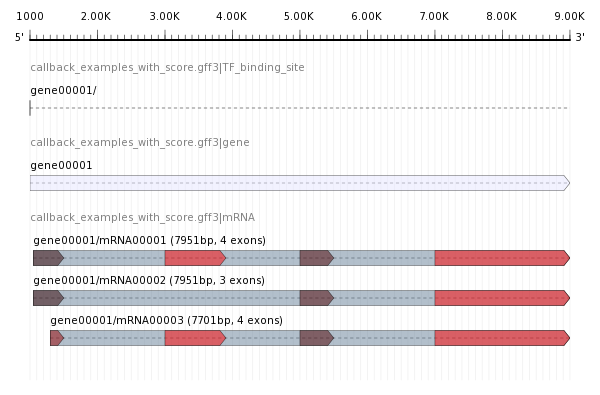
\includegraphics[width=.7\textwidth]{../../www/genometools.org/htdocs/images/callbacks}}
\caption{Example rendering of a GFF file using callback functions to enable custom block captions and score-dependent shading of exon features.}
\label{callbacks}
\end{figure}

\section{The \texttt{gt sketch} tool}

The \emph{GenomeTools} \texttt{gt} executable provides a new tool which uses the \emph{AnnotationSketch} library to create a drawing in PNG, PDF, PostScript or SVG format from GFF3 annotations. The annotations can be given by supplying one or more file names as command line arguments:
\small
\begin{verbatim}
$ gt sketch output.png annotation.gff3
$
\end{verbatim}
\normalsize
or by receiving GFF3 data via the standard input, here prepared by the \texttt{gt gff3} tool (here called with the \texttt{-addintrons} option to automatically add intron features between exons):
\small
\begin{verbatim}
$ gt gff3 -addintrons annotation.gff3 | gt sketch output.png
$
\end{verbatim}
\normalsize
The region to create a diagram for can be specified in detail by using the \texttt{-seqid}, \texttt{-start} and \texttt{-end} parameters. For example, if the \emph{D. melanogaster} gene annotation is given in the \texttt{dmel\_annotation.gff3} file, use
\small
\begin{verbatim}
$ gt sketch -format pdf -seqid 2R -start 9326816 -end 9332879 output.pdf \
  dmel_annotation.gff3
$
\end{verbatim}
\normalsize
to plot a graphical representation of the \emph{cnn} and \emph{cbs} gene region from the \emph{FlyBase} default view in PDF format.
The \texttt{-force} option can be used to force overwriting of an already existing output file. The \texttt{-pipe} option additionally allows passing the GFF3 input through the sketch tool via the standard output, allowing the intermediate visualisation of results in a longer pipeline of connected GFF3 tools. More command line options are available; their documentation can be viewed using the \texttt{-help} option.

If an input file file is not plotted due to parsing errors, \emph{GenomeTools} includes a strict GFF3 validator tool to check whether the input file is in valid GFF3 format. Simply run a command like the following:
\small
\begin{verbatim}
$ gt gff3validator input_file.gff3
input is valid GFF3
$
\end{verbatim}
\normalsize
This validator also allows to check the SO types occurring in a GFF3 file against a given OBO ontology file. This checking can be enabled by specifying the file as an argument to the \texttt{-typecheck} option.

\section{Examples}

This section will show how to use the \emph{AnnotationSketch} library in custom applications. As \emph{AnnotationSketch} is distributed as a part of \emph{GenomeTools}, its code is compiled into the \texttt{libgenometools.so} shared library. Please refer to the INSTALL file inside the \emph{GenomeTools} distribution for installation instructions.

For a general idea about how to use the library, a simple implementation of the GFF3 validator is included in the source package (see \texttt{src/examples/gff3validator.c}) as an example showing how to create \emph{GenomeTools}-based programs. In the same directory, there is also an appropriate \texttt{Makefile} to build and link this application against the installed shared library \texttt{libgenometools.so}.

\subsection{Using \emph{AnnotationSketch} to draw annotations from a file}
The following code examples (in C and Lua) illustrate how to produce an image from a given GFF3 file using \emph{AnnotationSketch}. The result is shown in Fig. \ref{parsed_img}. In essence, these code examples implement something like a simple version of the \texttt{gt sketch} tool from \emph{GenomeTools} without most command-line options. The C-based examples mentioned below are compiled along with the \emph{GenomeTools} library itself and available in the \texttt{bin/examples} directory.

\begin{figure}
\centering{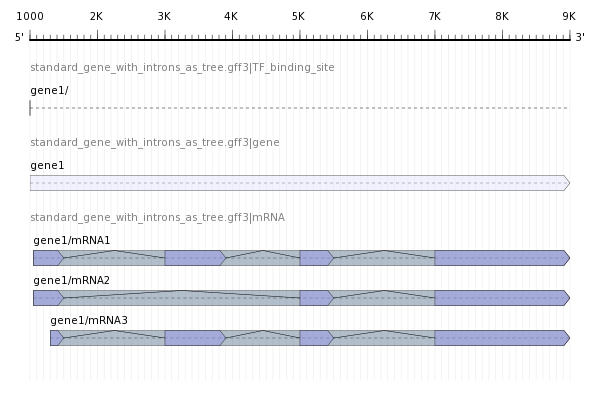
\includegraphics[width=.7\textwidth]{../../www/genometools.org/htdocs/images/parsed}}
\caption{Example rendering of a GFF3 file with default style.}
\label{parsed_img}
\end{figure}

\subsubsection{C code}
(See \texttt{src/examples/sketch\_parsed.c} in the source distribution.)
\lstinputlisting[language=C, breaklines=true, numbers=left, frame=single,]{../../src/examples/sketch_parsed.c}
\subsubsection{Lua code}
(See \texttt{gtscripts/sketch\_parsed.lua} in the source distribution. This example can be run by the command line \texttt{gt gtscripts/sketch\_parsed.lua <style\_file> <PNG\_file> <GFF3\_file>})
\lstinputlisting[language=Lua, breaklines=true, numbers=left, frame=single,]{../../gtscripts/sketch_parsed.lua}
\subsubsection{Ruby code}
(See \texttt{gtruby/sketch\_parsed.rb} in the source distribution.)
\lstinputlisting[language=Ruby, breaklines=true, numbers=left, frame=single,]{../../gtruby/sketch_parsed.rb}

\subsection{Using \emph{AnnotationSketch} to draw user-generated annotations}
The following C code example illustrates how to produce an image from annotation graphs created by user code.
 The result is shown in Fig. \ref{constructed_img}.

\begin{figure}
\centering{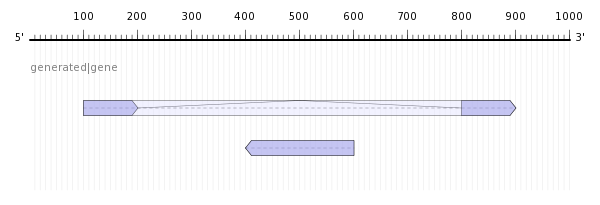
\includegraphics[width=.7\textwidth]{../../www/genometools.org/htdocs/images/constructed}}
\caption{Example rendering of user-generated annotations with default style.}
\label{constructed_img}
\end{figure}

\subsubsection{C code}
(See \texttt{src/examples/sketch\_constructed.c} in the source distribution.)
\lstinputlisting[language=C, breaklines=true, numbers=left, frame=single,]{../../src/examples/sketch_constructed.c}
\subsubsection{Lua code}
(See \texttt{gtscripts/sketch\_constructed.lua} in the source distribution.  This example can be run by the command line \texttt{gt gtscripts/sketch\_constructed.lua <style\_file> <PNG\_file>})
\lstinputlisting[language=Lua, breaklines=true, numbers=left, frame=single,]{../../gtscripts/sketch_constructed.lua}


\input{api_reference}
%\input{gtscript_reference}

\end{document}
